\section{Experimental Evaluation}
\label{sec:exp}

{\bf Experimental environment.} All experiments in this section were
conducted on an 8-slave in-house Open Stack cloud, using Linux Ubuntu
14.04 and Spark v1.4.  Each node has 4 cores and 16 GB of RAM.  Spark
Standalone cluster manager and Hadoop 2.6 were used.

Because Spark is a lazy evaluation system, a \insql{materialize}
operation was appended to the end of each query, which consisted of
the count of nodes and edges.  In cases where the goal was to evaluate
a specific operation in isolation, we used warm start, which consisted
of materializing the graph upon load.  Each experiment was conducted 3
times, we report the average running time, which is representative
because we took great care to control variability.  Standard deviation
for each measure is at or below 5\% of the mean except in cases of
very small running times.

{\bf Data.}  We evaluate performance of our framework on two real
open-source datasets.
%\begin{enumerate}%[leftmargin=*]
%\item 
DBLP~\cite{dblp} contains co-authorship information from 1936 through
2015, with over 1.5 million author nodes and over 6 million undirected
co-authorship edges.  Total data size: 250 MB.
%
nGrams~\cite{nGrams} contains word co-occurrence information from 1520
through 2008, with over 1.5 million word nodes and over 65 million
undirected co-occurrence edges.  Total data size: 40 GB.  

The nGrams dataset is of comparable size to the LiveJournal dataset
in~\cite{Xin2013} and is commensurate with our cluster size.  DBLP and
nGrams differ not only in size, but also in the evolutionary
properties: co-authorship network nodes and edges have limited
lifespan, while the nGrams network grows over time, with nodes and
edges persisting for long duration.  \eat{All figures in the body of this
section are on the larger nGrams dataset.  Refer to the Appendix for
the DBLP figures, which show similar trends as nGrams.}  We plan to
carry out further experiments with a larger
DELIS\footnote{\url{law.di.unimi.it/webdata/uk-union-2006-06-2007-05}}
dataset as we grow the cluster in the near future.

%\subsection{Degrees}

{\bf Degrees.} Computation of the number of edges for each vertex is
performed using a single round of message sending between nodes, with
batch mode for HG and OG.  We used the following query to evaluate
data structure performance over varying number of snapshots:

\begin{small}
\begin{verbatim}
      TSelect V[vid, degrees()];
              E[vid1, vid2]
      From    nGrams
      TWhere  Start >= x And End <= y
\end{verbatim}
\end{small}

\begin{figure*}[t]
\centering
\begin{minipage}{3in}
  \centering
  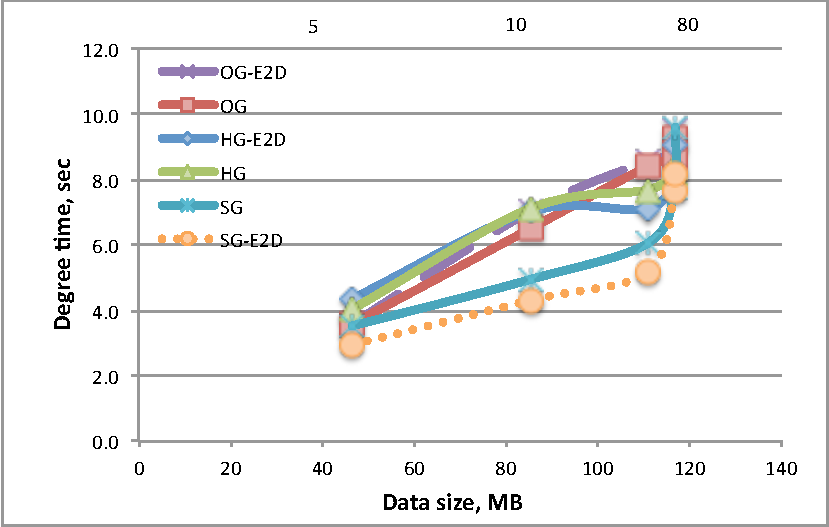
\includegraphics[width=2.6in]{figs/degrees_dblp.pdf}
  \vspace{-0.1in}
  \caption{Degrees time, dblp.}
  \label{fig:deg_dblp}
  \vspace{-0.1in}
\end{minipage}
\begin{minipage}{3in}
  \centering
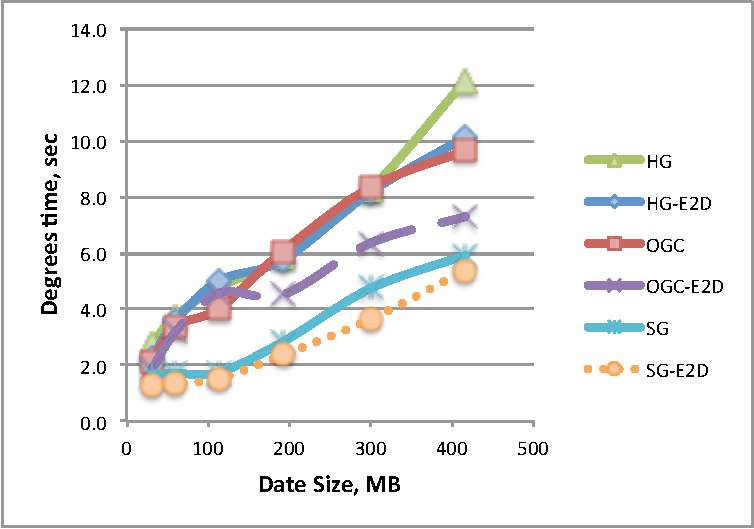
\includegraphics[width=2.6in]{figs/degrees_ngrams.pdf}
  \vspace{-0.1in}
\caption{Degrees time, nGrams.}
\label{fig:deg_ngrams}
  \vspace{-0.1in}
\end{minipage}
\end{figure*}

SG performs better than the other data structures in this experiment,
contrary to our expectation that batch mode of HG and OG would be
faster (Figures~\ref{fig:deg_dblp}, \ref{fig:deg_ngrams}, with warm
start).  SG performance can be explained if we consider that each
snapshot is spread out over fewer partitions than in the aggregate
data structures.  Thus, more communication occurs intra-partition
rather than between partitions.  Communication cost dominates the
overall running time.  Furthermore, we expected HG performance to be
between SG and OG, the two data structures that it combines.  We do
observe this in most cases, but not consistently.  We believe that HG
does not consistently outperform OG dues to its sensitivity to
temporal skew.  This effect is particularly pronounced for
fast-running operations like Degree.

%\subsection{Connected Components}

{\bf Connected components.} Snapshot analytics like Connected
  Components are implemented using the Pregel API in GraphX, with
  batch mode for HG and OG.  We used the following query to evaluate
  data structure performance over varying number of snapshots:

\begin{small}
\begin{verbatim}
      TSelect V[vid, components()];
              E[vid1, vid2]
      From    nGrams
      TWhere  Start >= x And End <= y
\end{verbatim}
\end{small}

\begin{figure*}[t]
\centering
\begin{minipage}{3in}
  \centering
  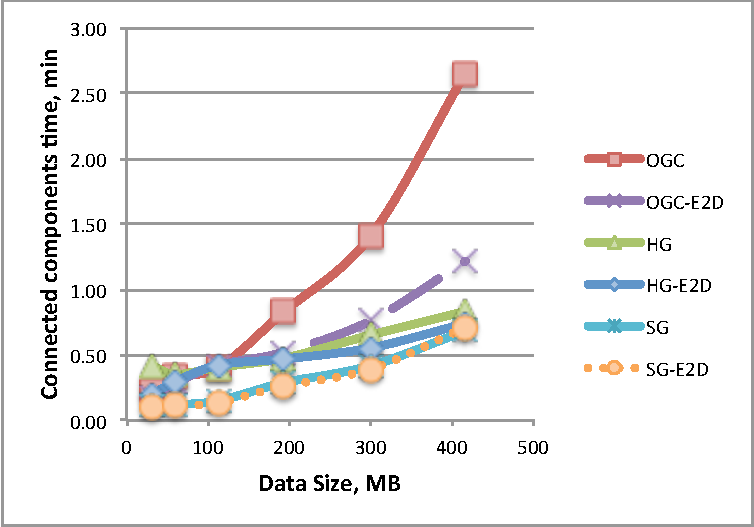
\includegraphics[width=2.6in]{figs/connectedcs_ngrams.pdf}
  \vspace{-0.1in}
  \caption{Connected Components, nGrams.}
  \label{fig:connectc_ngrams}
  \vspace{-0.1in}
\end{minipage}
\begin{minipage}{3in}
  \centering
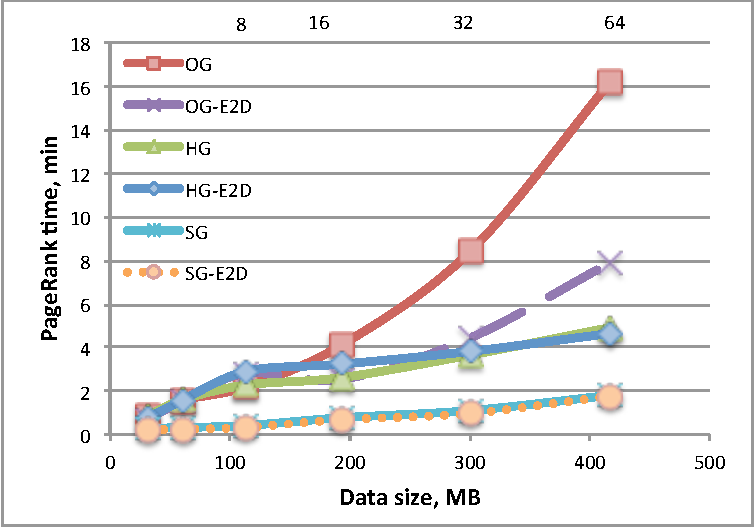
\includegraphics[width=2.6in]{figs/pagerank_ngrams.pdf}
  \vspace{-0.1in}
\caption{PageRank, nGrams.}
\label{fig:pagerank_ngrams}
  \vspace{-0.1in}
\end{minipage}
\end{figure*}

The algorithm was executed until convergence, with no limit to the
number of iterations.  Performance of Pregel-based algorithms depends
heavily on the partition strategy, with best results achieved where
cross-partition communication is small.  For this reason, we evaluated
only no partitioning and E2D.

SG performs better than the other data structures in this experiment,
contrary to our expectation that batch mode of HG and OG would be
faster (Figure~\ref{fig:connectedc_ngrams}).  This can be explained by
HG and OG using significantly more cross-partition communication due
to the following factors:

\begin{enumerate}[leftmargin=*]
\item Each individual snapshot is less dense than the aggregate
  (although this depends on the rate of change), and dense graphs do
  worse with Pregel analytics.
\item Individual snapshots are smaller and take fewer partitions, so
  less communication happens across partitions.
\item Each iteration gets faster as vertex values converge, because
  those vertices stop sending out new messages.  In OG/HG a vertex
  converges only when it does so in all snapshots of a batch.
  \eat{\item Messages for OG/HG are larger --- it is more costly to
    send a Map object than a number.}
\end{enumerate}

However, note that as the number of total snapshots increases, HG
performance improves compared to SG, and in fact for the largest size
(128) HG surpasses SG in performance.  We saw this trend in both data
sets.

%\subsection{PageRank}

{\bf PageRank.} PageRank is implemented using Pregel, like Connected
Components above.  The query is the same, replacing \insql{components}
with \insql{pagerank}.  PageRank was executed for 10 iterations or
until convergence, whichever came first.  The results of this
experiment (Figure~\ref{fig:pagerank_ngrams}) are similar to those of
the experiment above: SG outperforms the other data structures, but HG
exhibits the same slope and its performance improves relative to the
other data structures as the number of snapshots is increased.  E2D
partitioning leads to performance improvements for SG, but
inconsistent for HG/OG.

%\subsection{Mixed queries}

{\bf Mixed queries.} All the experiments so far evaluated performance
of individual \ql analytics operations.  We want to see what happens
when operations are combined in a single query such as this:

\begin{small}
\begin{verbatim}
      TSelect Any V[vid, trend(deg)];
              Any E
      From    (Tselect V[vid, degrees() as deg]; 
                       E[vid1, vid2]
               From    nGrams
               TWhere  Start >= x And End <= y)
      TGroup by size
\end{verbatim}
\end{small}

This query computes a degree of each vertex in each snapshot,
aggregates all snapshots into a single graph, and uses trend analytic
as the aggregation function on degrees.  We have shown above that in
most cases SG provides the most efficient performance for snapshot
analytics.  We have also shown in (under review) that aggregate data
structures (OG, HG, others) take longer to load but are more efficient
for a \insql{TGroup} operation.  When these operations are combined,
there is no significant difference in performance between SG and OG
(Figure~\ref{trend_deg} with cold start).  At this time we do not have
an implementation of temporal aggregation for HG.

\begin{figure*}[t]
\centering
\begin{minipage}{3in}
  \centering
  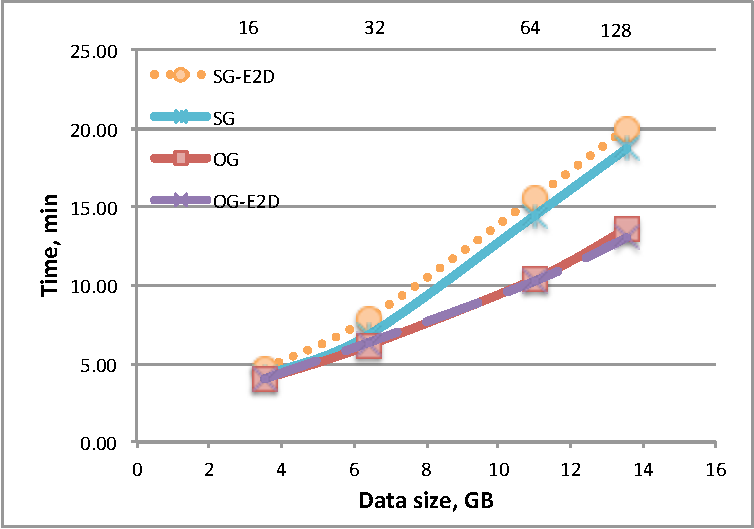
\includegraphics[width=2.6in]{figs/trend_degrees.pdf}
  \vspace{-0.1in}
  \caption{\insql{trend(degrees())}.}
  \label{fig:trend_deg}
  \vspace{-0.1in}
\end{minipage}
\begin{minipage}{3in}
  \centering
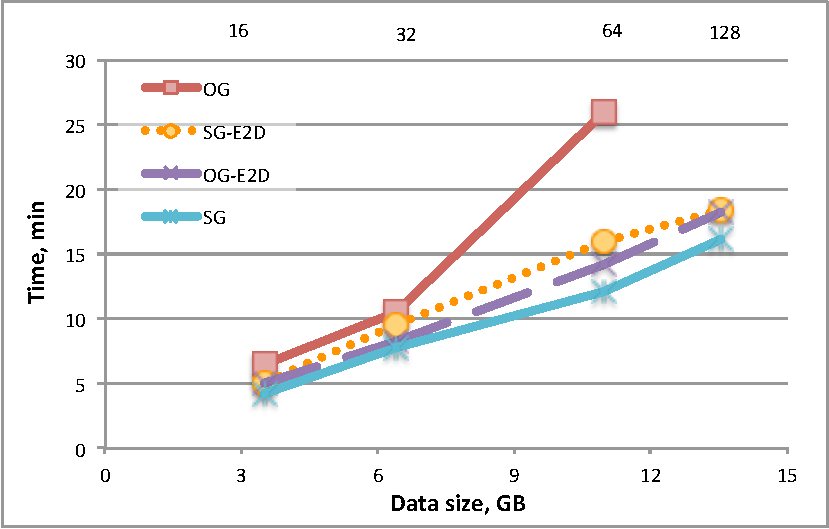
\includegraphics[width=2.6in]{figs/complexq.pdf}
  \vspace{-0.1in}
\caption{Complex query: \insql{TGroup}, PageRank, trend.}
\label{fig:complexq}
  \vspace{-0.1in}
\end{minipage}
\end{figure*}

\eat{
\subsection{\insql{TSelect} with \insql{trend(pagerank())}}
}

We conclude this section with a cold-start execution of
the query:

\begin{small}
\begin{verbatim}
      Select vid, pr
      From (TSelect Any V[vid, trend(prank) as pr]
                    Any E
            From (TSelect All V[vid, pagerank() as prank]; 
                          All E
                  From nGrams
                  TWhere Start >= x And End <= y
                  TGroup by 8 years)
            TGroup by size).toVerticesFlat()
      Order by pr
      Limit 10
\end{verbatim}
\end{small}

\eat{
As we saw above, SG outperforms other representations for data load
and for PageRank, while OGC is very efficient for temporal
aggregation.  This query combines all of these operations, and adds a
trend analytic, and a transformation of the vertices of the result
into a flat vertex relation.
}
SG with no partitioning, and OGC with E2D show comparable
performances, as seen in Figure~\ref{fig:complexq}.

\eat{
\begin{figure}[t]
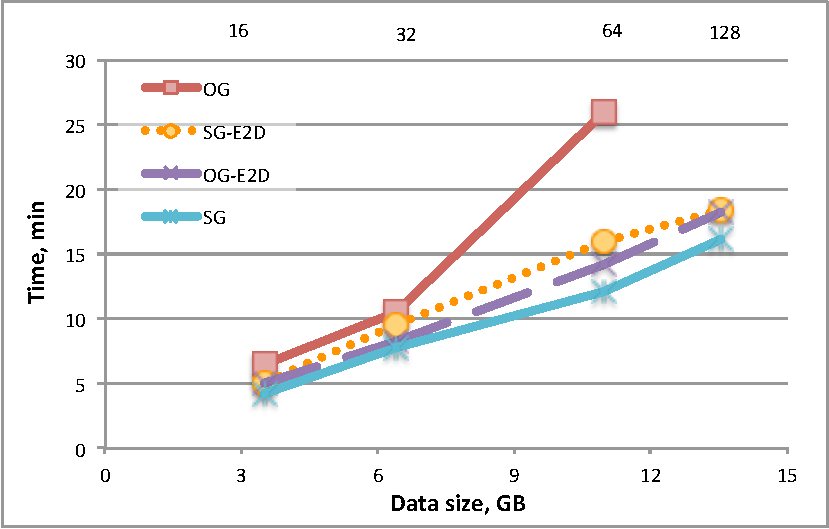
\includegraphics[width=3.2in]{figs/complexq.pdf}
\caption{Complex query: \insql{TGroup}, PageRank, trend.}
\label{fig:complexq}
\end{figure}
}

{\bf In summary,} no one data structure is most efficient across all
operations.  \eat{SG is most efficient for data load, because our file
  format favors this data structure, and for PageRank.  OGC is most
  efficient for temporal group and join.  The two data structures
  perform comparably for the complex query.  E2D is the most efficient
  partitioning method in most cases, and E2D-Temporal is a close
  second.}  SG is most efficient for snapshot analytics in most cases,
but HG provides a good balance for mixed queries.
